% ============================================================
% MSc Thesis Defense Slides
% "Cash Got Your Tongue? CEO Language-Uncertainty Around
%  Undisclosed Cash Acquisitions"
% Sina Soleimanipour, Telfer School of Management, uOttawa
%
% All coefficients verified byte-exact against
% docs/Thesis/_uottawa_rewrite/_tables_from_bible.tex (2026-07-09).
% Honesty floor (register locks) respected throughout:
%   correlational / within-firm / no identification / mechanism open /
%   concentration not strict specificity / GAP = indistinguishable
%   from zero once announced (never "falls") / stock = noisy null.
% Build: pdflatex defense_slides.tex (x2)
% ============================================================
\documentclass[aspectratio=169, 11pt]{beamer}

\usetheme{metropolis}
\setbeamertemplate{navigation symbols}{}
\setbeamertemplate{frame numbering}[fraction]

% Palette validated (dataviz six-checks, light surface):
% cash / uncertainty series = blue #2166AC; stock / cash-ratio = orange #E08214
\definecolor{cashblue}{HTML}{2166AC}
\definecolor{stockorange}{HTML}{E08214}
\definecolor{mutedgray}{HTML}{6B6B6B}

\usepackage{graphicx}
\usepackage{booktabs}
\usepackage{tikz}
\usepackage{pgfplots}
\pgfplotsset{compat=1.17}

\newcommand{\ns}{\textsuperscript{n.s.}}

\title{Cash Got Your Tongue?}
\subtitle{CEO Language-Uncertainty Around Undisclosed Cash Acquisitions}
\author{Sina Soleimanipour \\ MSc in Management (Finance), Thesis Defense}
\institute{Telfer School of Management, University of Ottawa \\[6pt]
  {\small Supervisors: Dr.\ Ali Akyol, Dr.\ Harshit Rajaiya \\
  Examiners: Dr.\ Shantanu Dutta, Dr.\ Rengong (Alex) Zhang}}
\date{2026}

\begin{document}

% ---------- 1. TITLE ----------
\begin{frame}[plain]
  \titlepage
\end{frame}

% ---------- 2. MOTIVATION ----------
\begin{frame}{Motivation: a firm that knows, but may not say}
  A firm privately committed to an acquisition it has not announced sits in a
  \alert{disclosure bind}:
  \begin{itemize}
    \item The pending deal can be \textbf{material} even while negotiations are
      preliminary (\textit{Basic v.\ Levinson}, 1988).
    \item The firm \textbf{may stay silent}: no general duty to disclose merger talks.
    \item But once it speaks, it \textbf{may not mislead} (Rule 10b-5): a flat
      denial is not a lawful option.
    \item Theory: informed managers may rationally withhold (Verrecchia 1983),
      and silence can survive in equilibrium (Dye 1985).
  \end{itemize}
  \vspace{0.5em}
  \begin{block}{The bind}
    The CEO must host the routine earnings call, cannot address the one material
    thing, and cannot deny it either. Does the spoken record track that withholding?
  \end{block}
\end{frame}

% ---------- 3. THIS PAPER ----------
\begin{frame}{This paper}
  \begin{center}
    \textbf{Research question:} does residual CEO Q\&A uncertainty track a deal's
    passage from \emph{private} to \emph{public}: elevated while a cash acquisition
    is withheld, receding once announced?
  \end{center}
  \vspace{0.3em}
  \textbf{Preview of findings} (all within-firm, correlational):
  \begin{itemize}
    \item Elevated in the quarter \emph{before} a cash acquisition; no comparable
      rise detected before stock acquisitions.
    \item Indistinguishable from zero once the deal is announced, even before
      completion, while the funding cash stays until closing.
    \item The elevation concentrates in cash deals; the difference survives a
      formal pooled test.
  \end{itemize}
  \vspace{0.2em}
  {\scriptsize\color{mutedgray} A descriptive regularity, read through disclosure
  theory: no causal identification, no tested mechanism.}
\end{frame}

% ---------- 4. MEASURE ----------
\begin{frame}{Measure: residual CEO Q\&A uncertainty (\textit{UncResCEO})}
  \textbf{Raw input:} share of uncertain language in the CEO's unscripted
  Q\&A answers on each earnings call.
  \vspace{0.4em}

  \textbf{Problem:} executives differ persistently in how tentatively they speak.
  A level comparison mixes \emph{style} with \emph{state}.
  \vspace{0.4em}

  \textbf{Solution} (decomposition following Dzielinski, Wagner, and Zeckhauser 2021):
  net out each executive's persistent speaking style; keep the
  \alert{call-varying residual}.
  \begin{itemize}
    \item \textit{UncResCEO} is centered near zero by construction;
      SD $= 0.3010$ (all-universe Table 1 basis).
    \item Computable only for CEOs with at least five calls at non-financial,
      non-utility firms (a coverage filter we disclose: it skews toward larger firms).
  \end{itemize}
  \vspace{0.3em}
  {\small\color{mutedgray} Details and estimating equations: backup slides.}
\end{frame}

% ---------- 5. DATA ----------
\begin{frame}{Data and sample}
  \begin{itemize}
    \item \textbf{Earnings calls:} Capital IQ transcripts, U.S.\ public,
      non-financial, non-utility firms, 2002--2018.
    \item \textbf{Deals:} SDC acquisitions; cash arm = at least half cash,
      stock arm = at least half stock (managed comparison).
    \item \textbf{Language sample:} 88{,}205 calls across 1{,}884 firms.
    \item \textbf{Cash-ratio panel} is broader (2{,}232 firms): the cash ratio
      needs no speaking-style residual.
    \item CashRatio $=$ cash and equivalents over assets; sample mean $0.1708$.
  \end{itemize}
  \vspace{0.5em}
  {\small\color{mutedgray} Every table reports its own firm and observation
  counts; the uncertainty regressions describe a better-covered,
  larger-firm subset.}
\end{frame}

% ---------- 6. DESIGN ----------
\begin{frame}{Empirical design: three main analyses}
  \begin{enumerate}
    \item \textbf{MA1, run-up:} two-way fixed-effects regression of
      \textit{UncResCEO} on a pre-announcement-quarter indicator; firm FE and
      calendar year-quarter FE. The firm is compared against itself.
    \item \textbf{MA2, event time:} matched sample around the announcement;
      windows PRE2, PRE1, GAP (announced, pre-close), POST (completed);
      same outcome pair: uncertainty and cash ratio.
    \item \textbf{MA3, cash-specificity:} both treatments pooled in one
      regression; the cash-minus-stock difference evaluated by a formal Wald test.
  \end{enumerate}
  \vspace{0.5em}
  \begin{itemize}
    \item Standard errors clustered by firm; focal tests read \textbf{two-tailed}.
    \item Post-announcement quarters dropped in the run-up design;
      never-acquirers form the baseline.
  \end{itemize}
\end{frame}

% ---------- 7. H1 RUN-UP ----------
\begin{frame}{H1: pre-announcement run-up (cash vs.\ stock)}
  \begin{columns}[T]
    \begin{column}{0.52\textwidth}
      \begin{center}
      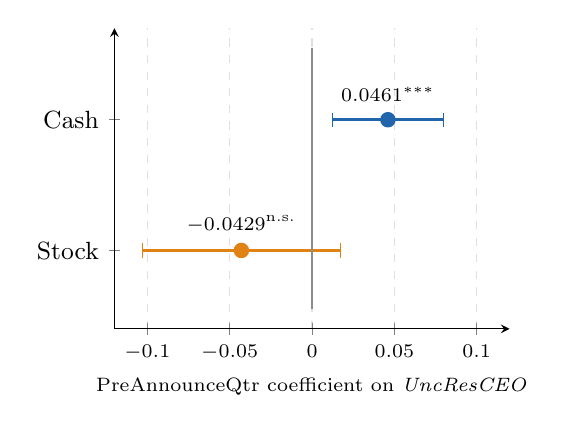
\begin{tikzpicture}
        \begin{axis}[
          width=6.6cm, height=5.4cm,
          xlabel={\scriptsize PreAnnounceQtr coefficient on \textit{UncResCEO}},
          ytick={0,1}, yticklabels={Stock, Cash},
          yticklabel style={font=\small},
          ymin=-0.6, ymax=1.7,
          xmin=-0.12, xmax=0.12,
          xtick={-0.10,-0.05,0,0.05,0.10},
          scaled x ticks=false,
          xticklabel style={font=\scriptsize, /pgf/number format/fixed,
            /pgf/number format/precision=2},
          axis x line=bottom, axis y line=left,
          every axis plot/.append style={only marks},
          xmajorgrids, grid style={dashed, black!12},
          clip=false,
        ]
          \addplot[color=cashblue, mark=*, mark size=2.6pt,
            mark options={fill=cashblue},
            error bars/.cd, x dir=both, x explicit,
            error bar style={line width=1.2pt, color=cashblue}]
            coordinates { (0.0461,1) +- (0.0337,0) };
          \addplot[color=stockorange, mark=*, mark size=2.6pt,
            mark options={fill=stockorange},
            error bars/.cd, x dir=both, x explicit,
            error bar style={line width=1.2pt, color=stockorange}]
            coordinates { (-0.0429,0) +- (0.0602,0) };
          \draw[black!45, line width=0.7pt]
            (axis cs:0,-0.45) -- (axis cs:0,1.55);
          \node[anchor=south, font=\scriptsize, yshift=3pt]
            at (axis cs:0.0461,1) {$0.0461^{***}$};
          \node[anchor=south, font=\scriptsize, yshift=3pt]
            at (axis cs:-0.0429,0) {$-0.0429$\ns};
        \end{axis}
      \end{tikzpicture}\\
      {\scriptsize 95\% CIs; firm-clustered SEs. Table: run-up test, cols.\ (2), (6).}
      \end{center}
    \end{column}
    \begin{column}{0.46\textwidth}
      \textbf{Cash acquirers:} $0.0461^{***}$ (SE $0.0172$; two-tailed
      $p=.0074$), about \textbf{15\% of a residual SD}. Material but modest.
      \vspace{0.5em}

      \textbf{Stock acquirers:} $-0.0429$, not significant (SE $0.0307$):
      a \alert{noisy flat null}, not a detected decline.
      \vspace{0.5em}

      {\small The firm's own cash ratio also drifts up pre-announcement
      ($0.0051^{***}$).}
      \vspace{0.5em}

      {\small\color{mutedgray} Within-firm, correlational.}
    \end{column}
  \end{columns}
\end{frame}

% ---------- 8. H1b EVENT TIME (STAR) ----------
\begin{frame}{H1b: the round trip in event time (matched sample)}
  \begin{center}
  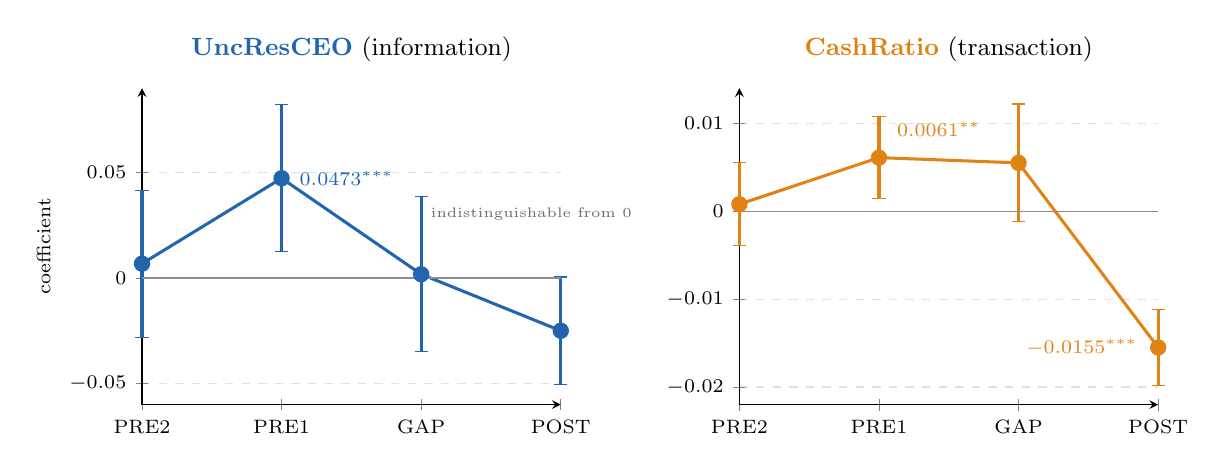
\begin{tikzpicture}
    \begin{axis}[
      name=unc,
      width=6.9cm, height=5.6cm,
      title={\small \textcolor{cashblue}{\textbf{UncResCEO}} (information)},
      symbolic x coords={PRE2, PRE1, GAP, POST},
      xtick=data, xticklabel style={font=\scriptsize},
      ymin=-0.06, ymax=0.09,
      scaled y ticks=false,
      yticklabel style={font=\scriptsize, /pgf/number format/fixed,
        /pgf/number format/precision=2},
      ylabel={\scriptsize coefficient}, ylabel near ticks,
      axis x line=bottom, axis y line=left,
      ymajorgrids, grid style={dashed, black!12},
      clip=false,
    ]
      \addplot[color=cashblue, mark=*, mark size=2.4pt, line width=1.1pt,
        error bars/.cd, y dir=both, y explicit,
        error bar style={line width=1.1pt}]
        coordinates {
          (PRE2,0.0068) +- (0,0.0349)
          (PRE1,0.0473) +- (0,0.0349)
          (GAP,0.0018)  +- (0,0.0367)
          (POST,-0.0250) +- (0,0.0255)
        };
      \draw[black!45] (axis cs:PRE2,0) -- (axis cs:POST,0);
      \node[anchor=west, font=\scriptsize, color=cashblue, xshift=3pt]
        at (axis cs:PRE1,0.0473) {$0.0473^{***}$};
      \node[anchor=south west, font=\tiny, color=mutedgray]
        at (axis cs:GAP,0.023) {indistinguishable from 0};
    \end{axis}
    \begin{axis}[
      at={(unc.outer east)}, anchor=outer west, xshift=6pt,
      width=6.9cm, height=5.6cm,
      title={\small \textcolor{stockorange}{\textbf{CashRatio}} (transaction)},
      symbolic x coords={PRE2, PRE1, GAP, POST},
      xtick=data, xticklabel style={font=\scriptsize},
      ymin=-0.022, ymax=0.014,
      scaled y ticks=false,
      yticklabel style={font=\scriptsize, /pgf/number format/fixed,
        /pgf/number format/precision=2},
      axis x line=bottom, axis y line=left,
      ymajorgrids, grid style={dashed, black!12},
      clip=false,
    ]
      \addplot[color=stockorange, mark=*, mark size=2.4pt, line width=1.1pt,
        error bars/.cd, y dir=both, y explicit,
        error bar style={line width=1.1pt}]
        coordinates {
          (PRE2,0.0008) +- (0,0.0047)
          (PRE1,0.0061) +- (0,0.0047)
          (GAP,0.0055)  +- (0,0.0067)
          (POST,-0.0155) +- (0,0.0043)
        };
      \draw[black!45] (axis cs:PRE2,0) -- (axis cs:POST,0);
      \node[anchor=south west, font=\scriptsize, color=stockorange,
        xshift=3pt, yshift=4pt]
        at (axis cs:PRE1,0.0061) {$0.0061^{**}$};
      \node[anchor=east, font=\scriptsize, color=stockorange, xshift=-4pt]
        at (axis cs:POST,-0.0155) {$-0.0155^{***}$};
    \end{axis}
  \end{tikzpicture}\\
  {\scriptsize Cash acquirers, matched sample; $N=28{,}102$ firm-quarters,
  1{,}320 firms; 95\% CIs, firm-clustered SEs. Two separate panels, one scale each.}
  \end{center}
\end{frame}

% ---------- 9. H1b TWO CLOCKS ----------
\begin{frame}{H1b: two clocks}
  \begin{columns}[T]
    \begin{column}{0.5\textwidth}
      \textbf{\textcolor{cashblue}{Information clock} (UncResCEO)}
      \begin{itemize}
        \item No pre-trend: PRE2 $0.0068$\ns
        \item Anticipatory rise: PRE1 $0.0473^{***}$
        \item \alert{Indistinguishable from zero once announced}: GAP $0.0018$\ns
        \item Drop PRE1$-$GAP $=0.0455^{**}$; PRE1$-$POST $=0.0723^{***}$
      \end{itemize}
    \end{column}
    \begin{column}{0.5\textwidth}
      \textbf{\textcolor{stockorange}{Transaction clock} (CashRatio)}
      \begin{itemize}
        \item Builds pre-announcement: PRE1 $0.0061^{**}$
        \item \textbf{Persists} while announced but unclosed (GAP)
        \item Leaves at completion: POST $-0.0155^{***}$;
          GAP$-$POST $=0.0210^{***}$
      \end{itemize}
    \end{column}
  \end{columns}
  \vspace{0.4em}
  \begin{block}{Reading}
    Uncertainty resolves on the \emph{information} clock (announcement); the
    funding cash resolves on the \emph{transaction} clock (completion). The
    elevation is anticipatory, not a reaction to the announcement.
  \end{block}
  \vspace{0.1em}
  {\scriptsize\color{mutedgray} POST uncertainty sits slightly below baseline
  ($-0.0250^{*}$); we do not over-read that overshoot. Cash persistence at
  closing is partly mechanical.}
\end{frame}

% ---------- 10. H1a CASH CONCENTRATION ----------
\begin{frame}{H1a: concentration in cash deals (formal pooled test)}
  \begin{columns}[T]
    \begin{column}{0.5\textwidth}
      Pooled regression, both treatments, one Wald restriction
      (two-tailed):
      \vspace{0.4em}
      \begin{center}
      \small
      \begin{tabular}{lc}
        \toprule
        & UncResCEO \\
        \midrule
        Pre-announce, Cash & $\mathbf{0.0459}^{**}$ \\
        & $(0.0185)$ \\
        Pre-announce, Stock & $-0.0524$\ns \\
        & $(0.0436)$ \\
        \midrule
        Cash $-$ Stock & $\mathbf{0.0983}^{**}$ \\
        & $(0.0476)$, $p=.039$ \\
        \bottomrule
      \end{tabular}
      \end{center}
    \end{column}
    \begin{column}{0.5\textwidth}
      \textbf{What we claim:} the run-up \alert{concentrates} in cash deals;
      the difference clears the five-percent bar in a formal test.
      \vspace{0.5em}

      \textbf{What we do not claim:}
      \begin{itemize}
        \item Not \emph{strict} specificity: significance rides on an
          imprecise stock arm, so the test is
          \textbf{supportive rather than definitive}.
        \item The proposed \emph{cause} is not cash-specific: the
          cash build-up difference is $0.0064$\ns\ (matched).
          \alert{The mechanism stays open.}
      \end{itemize}
    \end{column}
  \end{columns}
\end{frame}

% ---------- 11. RULE-OUTS ----------
\begin{frame}{Ruling out one alternative; one channel check}
  \textbf{Analyst cash-scrutiny (measured alternative driver).}
  Analysts do ask more cash questions pre-announcement; is the run-up just that?
  \begin{itemize}
    \item Run-up survives adding CashScrutiny and its interaction:
      PreAnnounceQtr $0.0413^{***}$; interaction $-0.0056$\ns.
    \item Hedge kept as in the thesis: measured scrutiny
      \alert{does not account for \emph{this} run-up}; we do not claim
      scrutiny never matters (the interaction test is underpowered).
  \end{itemize}
  \vspace{0.5em}
  \textbf{Bid-ask spread (information-asymmetry gauge).} Two per-component facts:
  \begin{itemize}
    \item The residual is \textbf{unrelated} to the post-call spread
      (n.s.\ in all 12 specifications).
    \item The \emph{scripted presentation} is positively associated with it
      (contemporaneous, one-tailed, within-firm).
    \item We report the two facts side by side; the between-component
      difference is \alert{not tested directly}.
  \end{itemize}
\end{frame}

% ---------- 12. ROBUSTNESS ----------
\begin{frame}{Robustness}
  The pattern holds qualitatively under:
  \begin{itemize}
    \item[\checkmark] \textbf{Withdrawal as resolution:} treating withdrawn
      deals' withdrawal date as the resolution event.
    \item[\checkmark] \textbf{Dropping the cash equation's dynamic term}
      (lagged CashRatio partial adjustment).
    \item[\checkmark] \textbf{All deals} (removing the first-deal restriction).
    \item[\checkmark] \textbf{Logit} variants of the linear specifications.
  \end{itemize}
  \vspace{0.6em}
  {\small\color{mutedgray} Full robustness tables in the thesis appendix;
  key fragments in the backup slides.}
\end{frame}

% ---------- 13. CONTRIBUTIONS ----------
\begin{frame}{Contributions (four, each descriptive)}
  To our knowledge, this thesis is the first to:
  \begin{enumerate}
    \item Read \textbf{residual Q\&A uncertainty} in the anticipatory window
      before an acquisition is public (nearest prior work reads managed tone,
      strategy vocabulary, and prices).
    \item Document that the pattern \textbf{concentrates in cash acquisitions},
      a contrast that survives a formal pooled test.
    \item Read the unscripted Q\&A as tracking a deal's
      \textbf{passage from private to public}, connecting withholding theory
      with transaction-anticipation evidence, while claiming no causal channel.
    \item Show the residual is \textbf{unrelated to the post-call bid-ask
      spread} while the scripted presentation is positively associated with it.
  \end{enumerate}
\end{frame}

% ---------- 14. LIMITATIONS ----------
\begin{frame}{Limitations (by design)}
  \begin{itemize}
    \item \textbf{Correlational, within-firm.} No causal identification;
      we characterize a regularity, we do not recommend acting on it.
    \item \textbf{Mechanism open.} Compliance-constrained speech and strategic
      reticence are observationally equivalent here; the cash build-up itself
      is not cash-specific (cause leg n.s.).
    \item \textbf{Stock arm is a noisy null}, not evidence of suppression;
      it is less precisely estimated (underpowered caveat).
    \item \textbf{Masking motivation} (stock acquirers manage the narrative)
      motivates the comparison; it is \emph{not} identified.
    \item \textbf{Selection:} the residual needs five calls per CEO, so the
      language sample skews toward larger, better-covered firms.
    \item \textbf{Generated regressand:} the residual is a first-stage output;
      we address inference in Ch.\ 2 (backup slide).
  \end{itemize}
\end{frame}

% ---------- 15. TAKEAWAYS ----------
\begin{frame}{Takeaways}
  \begin{enumerate}
    \item A constrained executive's unscripted answers carry a readable,
      \textbf{anticipatory} trace of an undisclosed cash acquisition.
    \item The trace is on the \textbf{information clock}: elevated before,
      indistinguishable from zero once announced; the funding cash stays
      until completion.
    \item It \textbf{concentrates in cash deals} (formal pooled test);
      concentration, not strict specificity; mechanism open.
  \end{enumerate}
  \vspace{1.2em}
  \begin{center}
    \Large Thank you.\\[0.4em]
    \normalsize Questions welcome.
  \end{center}
\end{frame}

% ============================================================
% BACKUP SLIDES
% ============================================================
\appendix

\begin{frame}[plain, noframenumbering]
  \begin{center}\Huge Backup slides\end{center}
\end{frame}

% ---------- B1. MA1 table ----------
\begin{frame}[noframenumbering]{Backup: run-up test (MA1), focal columns}
  \begin{center}
  \small
  \begin{tabular}{lcccc}
    \toprule
    & \multicolumn{2}{c}{Cash acquirers} & \multicolumn{2}{c}{Stock acquirers} \\
    \cmidrule(lr){2-3}\cmidrule(lr){4-5}
    & CashRatio & UncResCEO & CashRatio & UncResCEO \\
    \midrule
    PreAnnounceQtr & $\mathbf{0.0051}^{***}$ & $\mathbf{0.0461}^{***}$ & $-0.0036$ & $-0.0429$ \\
    & $(0.0017)$ & $(0.0172)$ & $(0.0035)$ & $(0.0307)$ \\
    \midrule
    Firm FE, Year-Qtr FE & Yes & Yes & Yes & Yes \\
    N (firm-quarters) & 67{,}590 & 27{,}622 & 84{,}979 & 39{,}377 \\
    Firms & 2{,}232 & 1{,}248 & 2{,}281 & 1{,}338 \\
    $R^2$ & 0.665 & 0.001 & 0.672 & 0.001 \\
    \bottomrule
  \end{tabular}
  \end{center}
  \vspace{0.4em}
  {\scriptsize Firm-clustered SEs; controls included (leverage, size, Tobin's Q,
  ROA, capex, dividend dummy, scaled CFO; lagged CashRatio in the cash-ratio
  equations). Never-acquirers form the baseline; post-announcement quarters
  dropped. Two-tailed stars. Full table: thesis, run-up test.}
\end{frame}

% ---------- B2. MA2 table ----------
\begin{frame}[noframenumbering]{Backup: event-time estimates (MA2), matched sample}
  \begin{center}
  \footnotesize
  \begin{tabular}{lcc}
    \toprule
    & (1) UncResCEO & (2) CashRatio \\
    \midrule
    PRE2 (pre-trend) & $0.0068$ & $0.0008$ \\
    & $(0.0178)$ & $(0.0024)$ \\
    PRE1 (pre-announce) & $\mathbf{0.0473}^{***}$ & $\mathbf{0.0061}^{**}$ \\
    & $(0.0178)$ & $(0.0024)$ \\
    GAP (announced, pre-close) & $0.0018$ & $0.0055$ \\
    & $(0.0187)$ & $(0.0034)$ \\
    POST (completed) & $\mathbf{-0.0250}^{*}$ & $\mathbf{-0.0155}^{***}$ \\
    & $(0.0130)$ & $(0.0022)$ \\
    \midrule
    Drop: PRE1 $-$ GAP & $\mathbf{0.0455}^{**}$ & $0.0006$ \\
    Drop: GAP $-$ POST & $0.0268$ & $\mathbf{0.0210}^{***}$ \\
    Drop: PRE1 $-$ POST & $\mathbf{0.0723}^{***}$ & $\mathbf{0.0216}^{***}$ \\
    \midrule
    N (firm-quarters); Firms & 28{,}102; 1{,}320 & 28{,}102; 1{,}320 \\
    \bottomrule
  \end{tabular}
  \end{center}
  {\scriptsize Firm and year-quarter FE; controls included; firm-clustered SEs;
  two-tailed stars.}
\end{frame}

% ---------- B3. MA3 table ----------
\begin{frame}[noframenumbering]{Backup: cash-specificity test (MA3)}
  \begin{center}
  \small
  \begin{tabular}{lccc}
    \toprule
    & EFFECT & \multicolumn{2}{c}{PROPOSED CAUSE} \\
    \cmidrule(lr){2-2}\cmidrule(lr){3-4}
    & UncResCEO & CashRatio & CashRatio \\
    & (matched) & (matched, +lag) & (full panel, +lag) \\
    \midrule
    Pre-announce, Cash & $\mathbf{0.0459}^{**}$ & $\mathbf{0.0056}^{**}$ & $\mathbf{0.0049}^{***}$ \\
    & $(0.0185)$ & $(0.0025)$ & $(0.0019)$ \\
    Pre-announce, Stock & $-0.0524$ & $-0.0008$ & $-0.0043$ \\
    & $(0.0436)$ & $(0.0066)$ & $(0.0051)$ \\
    \midrule
    Cash $-$ Stock (Wald) & $\mathbf{0.0983}^{**}$ & $0.0064$ & $\mathbf{0.0092}^{*}$ \\
    & $(0.0476)$ & $(0.0071)$ & $(0.0055)$ \\
    \midrule
    N; Firms & 25{,}600; 1{,}191 & 24{,}347; 1{,}176 & 61{,}876; 2{,}141 \\
    \bottomrule
  \end{tabular}
  \end{center}
  {\scriptsize Pooled: 837 first cash acquirers, 282 first stock acquirers;
  baseline = firms doing neither. Firm and year-quarter FE; firm-clustered SEs;
  two-tailed. EFFECT is cash-concentrated ($p=.039$); the proposed CAUSE
  (cash build-up) is not (matched leg n.s.), so the mechanism stays open.}
\end{frame}

% ---------- B4. DWZ construction ----------
\begin{frame}[noframenumbering]{Backup: constructing \textit{UncResCEO}}
  \begin{enumerate}
    \item For each call, measure the uncertainty share of the CEO's Q\&A
      answers (uncertain-word counts over words, Loughran-McDonald style
      lexicon; Ch.\ 2, eq.\ for \textit{UncAns}).
    \item Decompose following Dzielinski, Wagner, and Zeckhauser (2021):
      regress the call-level measure on executive fixed effects (persistent
      speaking style) plus controls including the scripted-presentation
      uncertainty (\textit{UncPreCEO}).
    \item \textit{UncResCEO} $=$ the residual: the \textbf{call-varying}
      component of CEO answer uncertainty.
  \end{enumerate}
  \vspace{0.5em}
  \textbf{Why residual, not level:} levels compare tentative speakers to
  confident ones; the residual compares each CEO to \emph{their own} baseline.
  \vspace{0.2em}

  {\scriptsize Requires at least five calls per CEO. Convergent validity: the
  residual co-moves positively with political-risk and policy-uncertainty
  measures (one-tailed tests; economic magnitudes modest; disclosed in Ch.\ 2).}
\end{frame}

% ---------- B5. Variable defs ----------
\begin{frame}[noframenumbering]{Backup: \textit{HighCash} vs.\ \textit{HighCashScrutiny}}
  Two distinct indicators; not interchangeable:
  \vspace{0.4em}
  \begin{itemize}
    \item $\textit{HighCash} = \mathbf{1}[\textit{CashRatio} \ge p67]$:
      top \textbf{tercile} of winsorized (1/99) CashRatio; sample mean $0.3333$.
      Used as a regressor only in the scrutiny-validity table.
    \item $\textit{HighCashScrutiny} = \mathbf{1}[\textit{CashScrutiny} > \text{median}]$:
      the median is 0, so it flags \textbf{any} cash scrutiny
      ($\approx 11\%$ of calls; mean $0.1127$).
  \end{itemize}
  \vspace{0.5em}
  \textbf{Scrutiny measure is real:} a firm's cash position predicts cash
  scrutiny (CashRatio $0.7530^{***}$ / $0.8519^{***}$; HighCash
  $0.1754^{***}$ / $0.1921^{***}$; one-tailed for the cash coefficient),
  yet scrutiny does not move the residual
  ($-0.0000$\ns\ OLS; $-0.0003$\ns\ logit, channel table).
  \vspace{0.4em}

  {\small \textit{CashRatio} $=$ cash and equivalents (cheq) over total assets (atq).}
\end{frame}

% ---------- B6. Generated regressand ----------
\begin{frame}[noframenumbering]{Backup: generated-regressand inference}
  \textbf{Concern:} \textit{UncResCEO} is a first-stage residual used as the
  dependent variable downstream (Pagan 1984 class of problems).
  \vspace{0.5em}
  \begin{itemize}
    \item Addressed in Ch.\ 2 (measure construction and estimating equations):
      the first stage is estimated on the full call panel, and downstream
      regressions treat the residual as data.
    \item Because the generated variable is the \emph{regressand} (not a
      regressor), coefficient estimates downstream are not biased by the
      construction; the first-stage sampling error inflates the outcome's
      noise, which works \emph{against} finding the run-up.
    \item Focal results are read two-tailed and survive
      (run-up $p=.0074$; timing and cash-specificity tables are two-tailed).
  \end{itemize}
\end{frame}

% ---------- B7. Gelman-Stern ----------
\begin{frame}[noframenumbering]{Backup: why a formal pooled test (not side-by-side stars)}
  \textbf{Gelman and Stern (2006):} the difference between ``significant'' and
  ``not significant'' is not itself statistically significant.
  \vspace{0.5em}
  \begin{itemize}
    \item So we \textbf{never} claim cash-specificity from
      ``cash is starred, stock is not.''
    \item Instead MA3 pools both treatments and tests the
      \textbf{difference directly}: $0.0983$ (SE $0.0476$), $p=.039$,
      two-tailed Wald.
    \item That is also why the claim stays at \emph{concentration}:
      the difference clears 5\%, but its significance rides on the imprecise
      stock arm ($-0.0524$, SE $0.0436$), so: supportive rather than definitive.
  \end{itemize}
\end{frame}

% ---------- B8. Why cash ----------
\begin{frame}[noframenumbering]{Backup: why cash deals, not stock?}
  \textbf{Motivation, not identification:}
  \begin{itemize}
    \item A stock acquirer's currency is its own price, so it has an incentive
      to \emph{manage the narrative} rather than fall silent; a cash acquirer
      has no such currency to defend, and secrecy protects the deal.
    \item This masking asymmetry motivates comparing cash against stock;
      the thesis \textbf{does not identify} it as the operative channel.
  \end{itemize}
  \vspace{0.5em}
  \textbf{What the data say:}
  \begin{itemize}
    \item Cash arm rises ($0.0461^{***}$); stock arm is a noisy flat null
      ($-0.0429$\ns): \alert{the gap is cash rising, not stock suppressed}.
    \item Formal difference $0.0983^{**}$ ($p=.039$): concentration.
    \item The stock arm is less precisely estimated (SE $0.0307$ vs.\ $0.0172$):
      an underpowered-comparison caveat we keep.
  \end{itemize}
\end{frame}

% ---------- B9. Scrutiny detail ----------
\begin{frame}[noframenumbering]{Backup: cash-scrutiny detail}
  Three-step logic (all firm and year-quarter FE, firm-clustered):
  \begin{enumerate}
    \item \textbf{The confound is real:} scrutiny itself rises pre-announcement
      (HighCashScrutiny $0.0408^{**}$, run-up table col.\ 4).
    \item \textbf{The measure is valid:} a firm's cash position predicts cash
      questions (CashRatio $0.7530^{***}$ / $0.8519^{***}$, one-tailed).
    \item \textbf{But it does not carry the run-up:} adding CashScrutiny and
      its interaction leaves PreAnnounceQtr at $0.0413^{***}$;
      interaction $-0.0056$\ns\ (CI roughly $[-0.027, +0.016]$).
  \end{enumerate}
  \vspace{0.5em}
  \textbf{Honest bound:} a null-only rule-out; about 89\% of calls draw no cash
  scrutiny, so the interaction is underpowered. We claim only that measured
  scrutiny does not account for \emph{this} run-up.
\end{frame}

% ---------- B10. Robustness detail ----------
\begin{frame}[noframenumbering]{Backup: robustness inventory}
  \begin{itemize}
    \item \textbf{Withdrawal as resolution} (Ch.\ 4): withdrawn deals resolve
      uncertainty at withdrawal; pattern consistent.
    \item \textbf{Dropping the dynamic term:} cash-ratio equation without the
      lagged partial-adjustment term; conclusions unchanged.
    \item \textbf{All deals:} removing the first-deal restriction; pattern holds.
    \item \textbf{Logit variants:} binary high-uncertainty outcomes; consistent.
    \item Four robustness tables plus two logit tables in the thesis
      (\texttt{\_robustness\_tables.tex}).
  \end{itemize}
  \vspace{0.5em}
  {\small\color{mutedgray} Numbers quoted in the defense stay qualitative here;
  exact cells are in the thesis tables.}
\end{frame}

\end{document}
